\section{Turing-Completeness of a Language}
\label{sec:Turing Completeness}
In the dawn of computer science there were serveral ideas what computable 
means. Does it mean, that a machine can compute it, as Turing suggested? Or 
should we define some functions that should be computable and how they can be
combined to discuss the computability of a problem?

As it turned out, it does not matter -- the problems that can be solved in 
each of them are the same. This was shown by proving that the different 
mechanisms can simulate each other. By extension, a new formulism only needs 
to be able to simulate any of the existing formalisms to be at least as 
powerful as any of them. Thus came the expression \emph{Turing complete} to 
describe, that a certain formalism can build any Turing machine.

This chapter is build as exercises, because solving the problems gives a good 
impression, how one could go about proving other things to be turing complete.

\subsection{The Turing Machine}
The Turing Machine (\TM) is a formalism that focuses on a possible physical 
implementation of a computing machine, although far from what is used today. 
It features an potentially infinite amount of tape on which the machine 
operates and which it uses as storage. From this tape, the machine can read and
write the current cell and move its read-write-head one cell to the left or the
right. Finally, the machine has a finite number of ``states of mind",
comparable to a finite state automaton.

In order to formally analyse the \TM, we can code what such a machine would 
do in the following way:

\begin{defn}
	\label{def:tm}
	A Turing Machine $T$ is a tuple $(Q, \Sigma, \Gamma, \delta, q_0, q_{accept}, q_{reject})$
	where 
	\begin{itemize}
		\item $Q$ are the states of mind the machines can be in.
		\item $\Gamma$ is the tape alphabet, that can be used during the computation.
		\item $\Sigma\subset \Gamma$ is the input alphabet, of which the initial tape is a word.
		\item $\delta:Q\times \Gamma \rightarrow Q\times \Gamma\times \{L, N, R\}$ 
			is the transition function, which codes, how the \TM reacts to a state 
			and the current symbol -- i.e.\ what will be the new state of mind, what 
			symbol will be written and in which direction the head will move.
		\item $q_0\in Q$ gives the initial state.
		\item $q_{accept}, q_{reject}\in Q$ signify that the machine has stopped --
			successfully or not.
	\end{itemize}

	To run a \TM means to give it a word $w\in\Sigma^*$, place the head at some 
	cell on the tape and then execute the transitions indicated by the transition
	function until we get into any of the states $q_{accept}$ or $q_{reject}$.

	A \emph{configuration} of a turing machine is then a tuple 
	$(l, c, r, s) \in \Gamma^*\times \Gamma \times \Gamma^*\times Q$ 
	and we have 
	\begin{equation*}
		\interpret[\TM]{T}(l, c, r, s) = \begin{cases}
			(l, c, r, s), &\text{ if } s \in \{q_{accept}, q_{reject}\} \\
			(l, \tilde{c}, r, \tilde{s}) , &\text{ if } \delta(s,c) = (\tilde{s}, \tilde{c}, N)\\
			(\tilde{c}\, l , first(r), rest(r), \tilde{s}) , &\text{ if } \delta(s,c) = (\tilde{s}, \tilde{c}, R)\\
			(rest(l), first(l), \tilde{c}\, r, \tilde{s}) , &\text{ if } \delta(s,c) = (\tilde{s}, \tilde{c}, L)
		\end{cases}
	\end{equation*}

	\begin{figure}[htb]
		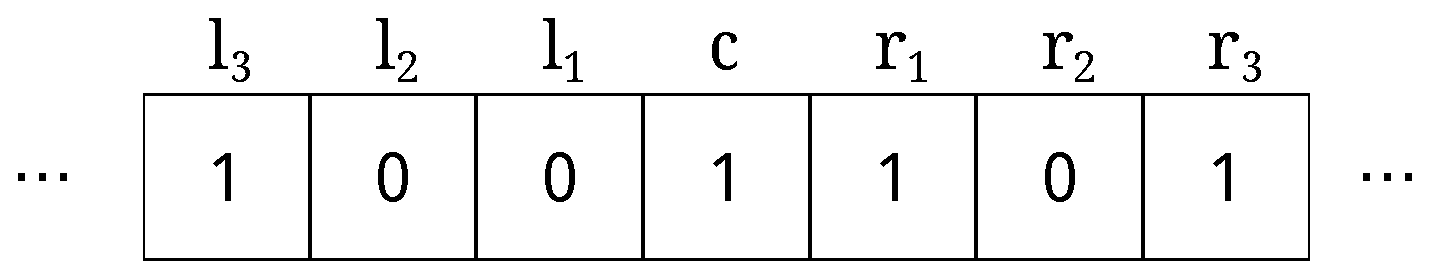
\includegraphics[width=0.95\textwidth]{computability/completeness/pictures/turingtape}
		\caption{Tape of the turing machine}
	\end{figure}
\end{defn}

\begin{example}[Adding two binary numbers]
	When we implement binary addition, we first need to think about how to 
	represent the problem. One of the easiest way to do that is to use {\tt 0} 
	and {\tt 1} to represent the digits, {\tt +} to separate the arguments, 
	{\tt =} ending the tape and assume that the numbers start with the least
	significant number on the left (which is the reverse of the usual notation,
	but easier to calculate with).
	
	\begin{algorithmic}[1]
		\State Start with $carry=0$ in mind.
		\If {tape shows 0}
				\State keep same $carry$ in mind
		\ElsIf {tape shows 1} 
			\If {$carry=0$}
				\State have $carry=1$ in mind
			\ElsIf {$carry=1$}
				\State have $carry=2$ in mind
			\EndIf
		\ElsIf {tape shows +}
			\State keep same $carry$ in mind
			\State have $finished = 1$ in mind
		\EndIf
		\State Move to the right until you hit {\tt +}.
		\If {tape shows 0}
				\State keep same $carry$ in mind
		\ElsIf {tape shows 1}
			\If {$carry=0$}
				\State have $carry=1$ in mind
			\ElsIf {$carry=1$}
				\State have $carry=2$ in mind
			\ElsIf {$carry=2$}
				\State have $carry=3$ in mind
			\EndIf
		\ElsIf {tape shows +}
			\State keep same $carry$ in mind
			\If {$finished=1$}
				\State have $finished = 2$ in mind
			\EndIf
		\EndIf
		\State Move to the right until you hit {\tt =}.
		\State Move to the right until you hit \#.
		\If {$carry=0$}
			\State write {\tt 0}
			\State have $carry=0$ in mind
		\ElsIf {$carry=1$}
			\State write {\tt 1}
			\State have $carry=0$ in mind
		\ElsIf {$carry=2$}
			\State write {\tt 0}
			\State have $carry=1$ in mind
		\ElsIf {$carry=3$}
			\State write {\tt 1}
			\State have $carry=1$ in mind
		\EndIf
		\If {$finished=2$}
			\State You're done
		\Else
			\State move to the far left
		\EndIf
	\end{algorithmic}
	The following shows the state transitions for the main loop of this 
	algorithm, the number of states would nearly double, if the $finished$ 
	states would be taken into account.

	\begin{center}
		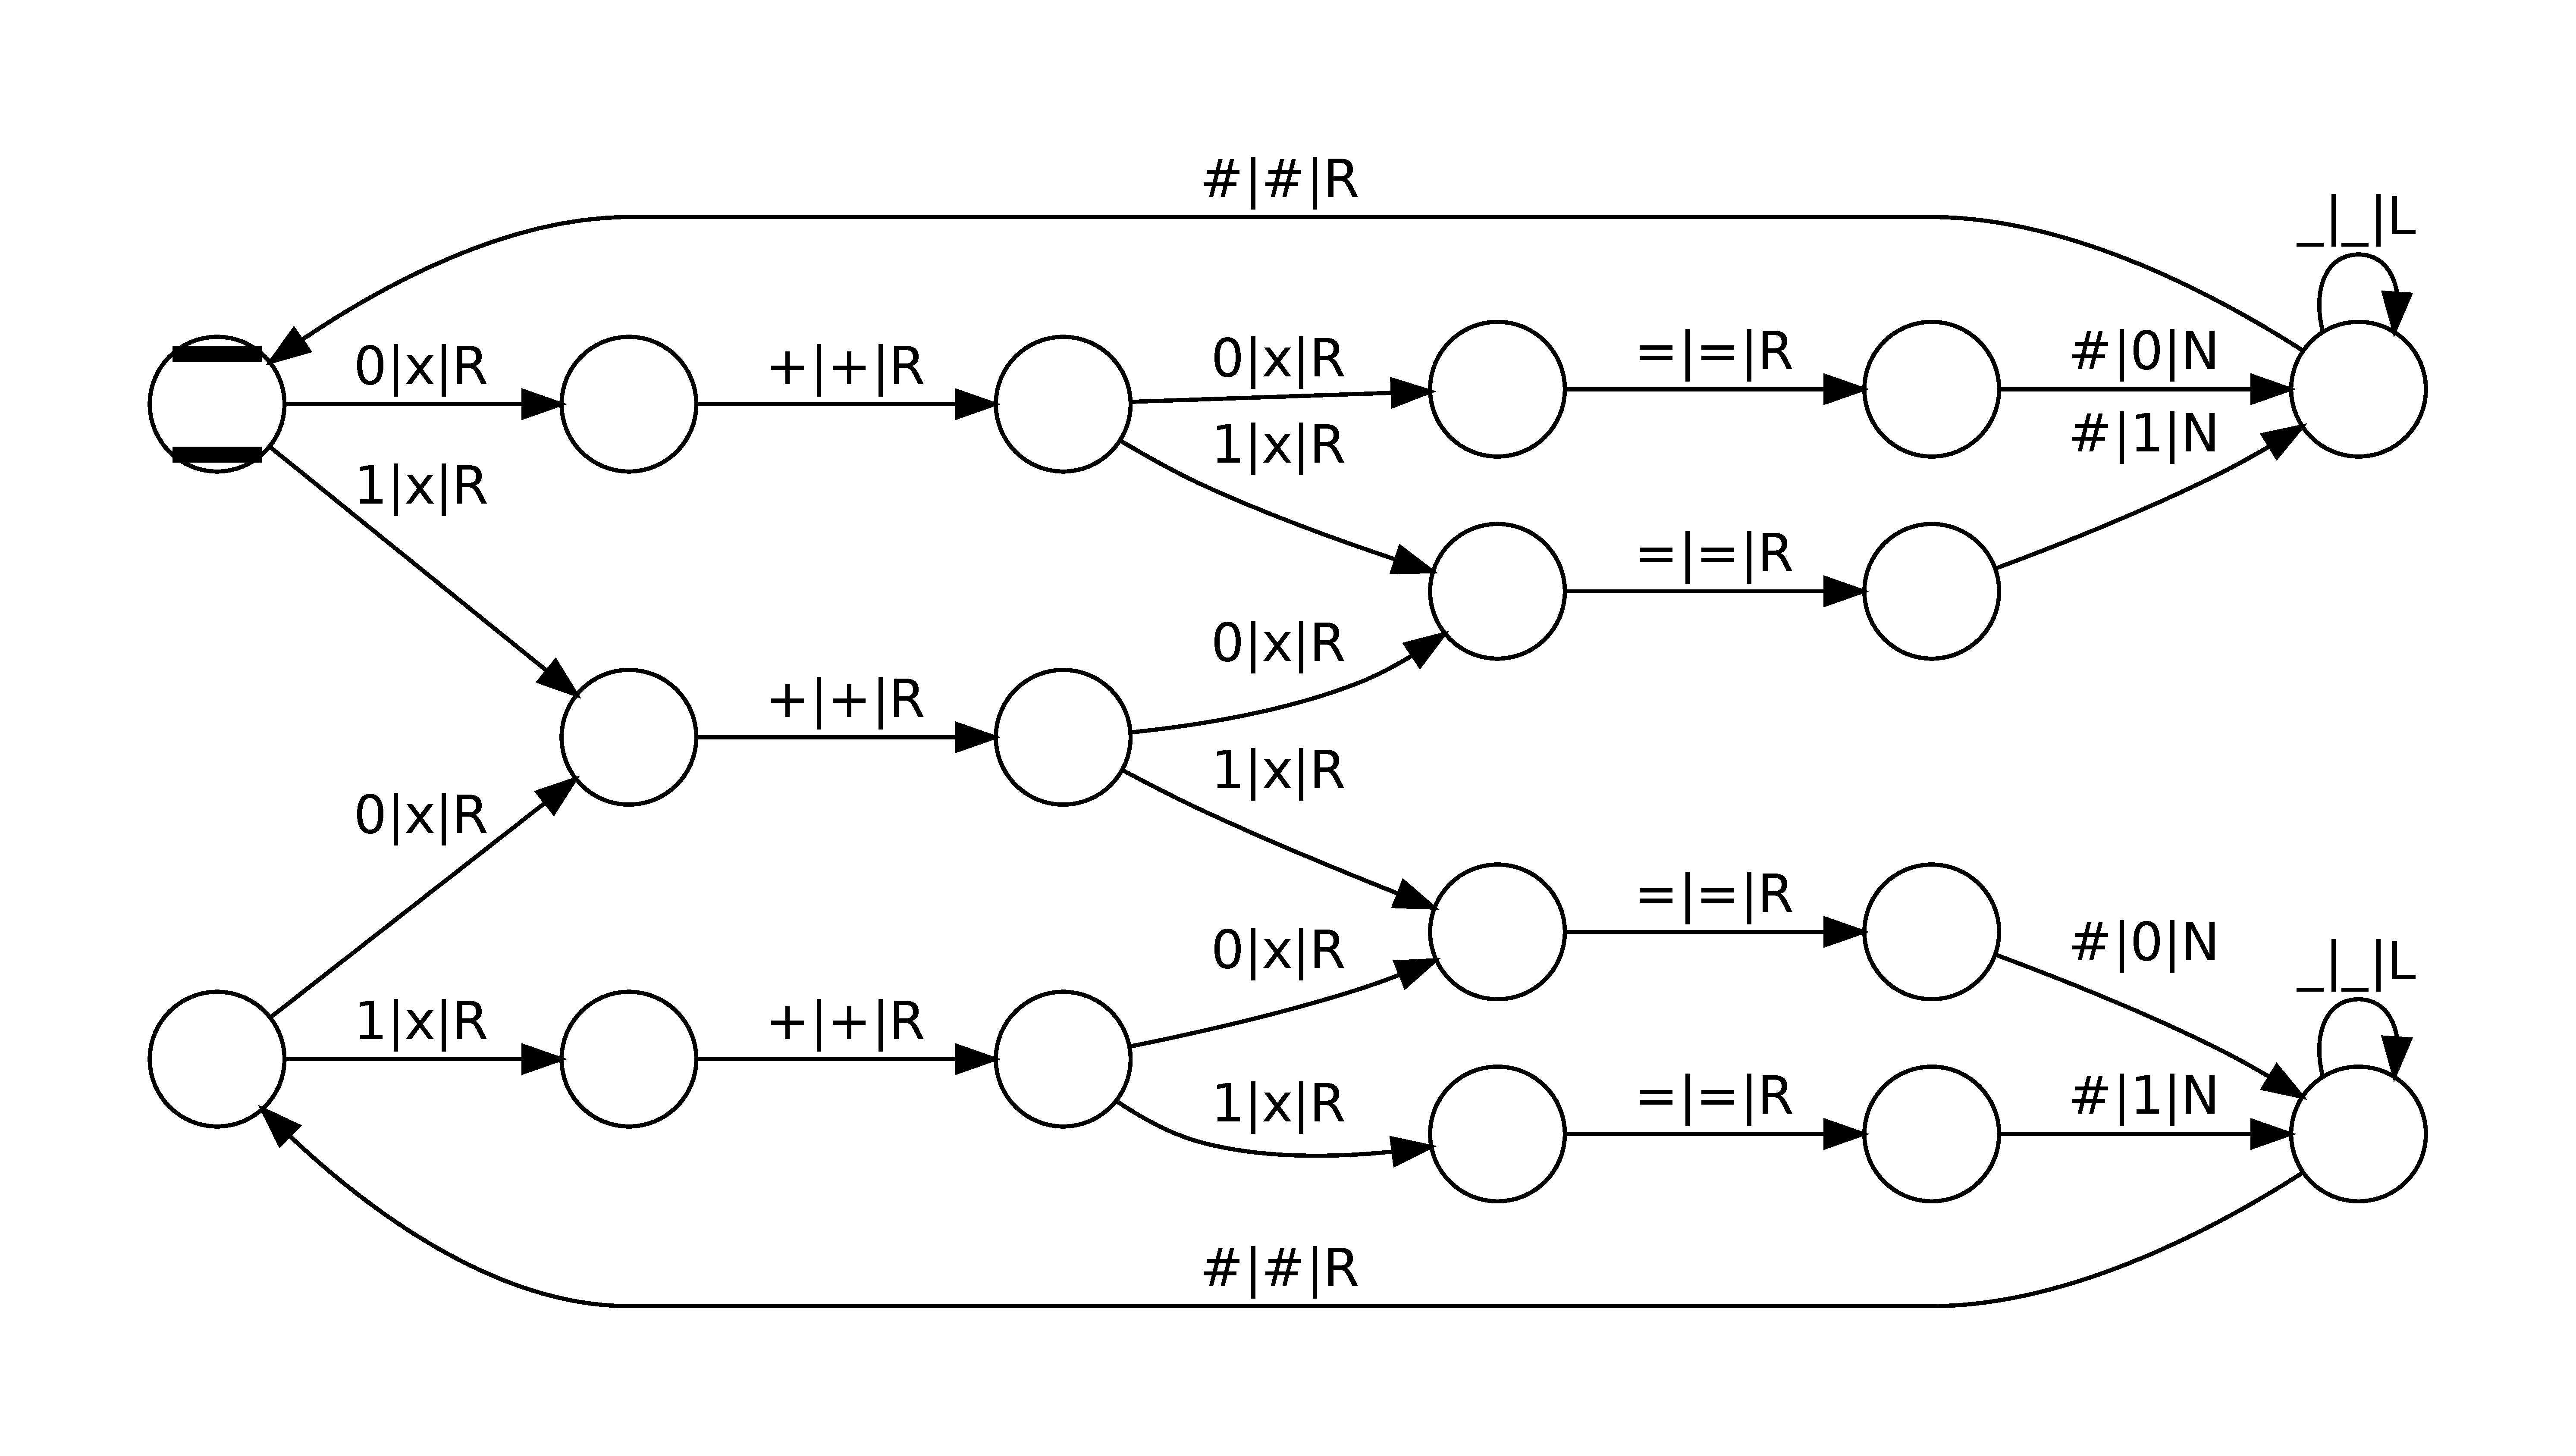
\includegraphics[width=0.99\textwidth]{computability/completeness/pictures/binary-adder}
	\end{center}
\end{example}

Seeing how complex turing machines get, it seems surprising, that it can code 
any machine or language.

\subsection{\WHILE is Turing complete}
By definition~\ref{def:power}, we would need a compiler from \TM to \WHILE, 
but by~\ref{thm:power-interpreter}, an interpreter suffices. Implementing such an 
interpreter will be the following exercise.

\begin{Exercise}[title={Interpreter for \TM},label={exc:tm},difficulty=2]
	\Question Show that we can implement a dictionary datastructure in \WHILE\@.
		Implement {\tt insert} and {\tt lookup}.
	\Question Show how you can code the transition function in your map.
	\Question Implement the tape
		\subQuestion Can you keep track of your position in a list with two stacks?
		\subQuestion Implement the left and right movement 
		$\interpret{{\tt left}},\interpret{{\tt right}} : Tape \rightarrow Tape$. Note that the list is 
			only potentially infinite, so you might in actuality run into the current edge.
	\Question Plug the pieces together to implement an interpreter {\tt turing(TM)} for turing machines.
		\subQuestion How many nested {\tt while} loops do you need?
\end{Exercise}
\begin{Answer}
	\Question Since execution time is not an issue, we can implement this as a 
	list of pairs:

\begin{verbatim}
    lookup read (Table.Key) {
      for (K.Value) in Table {
        if [and](K = Key . [not](Result)) {
          Result := Value
        }
      }
    } Write Result

    insert read (Table.(Key.Value)) {
      Outtable := Nil
      for (K.V) in Table {
        if K = Key {
          Outtable := cons (Key.Value) Outtable
        }
        else {
          Outtable := cons (K.V) Outtable
        }
      }
    } write Outtable
\end{verbatim}

If you wanted to get rid of the copying of the whole list, you could also 
just prepend the new pair, since the lookup takes the first match.
	\Question The transition function 
	$\delta: TapeAlphabet \times State \rightarrow TapeAlphabet \times State\times \{L,N,R\}$
	can be coded by taking the alphabet and the states as symbols (or numbers) 
	and storing {\tt ((in-letter.in-state).(out-letter.out-state.direction))} 
	in the map {\tt M}. Now $\delta = \interpret{spec}(lookup.M)$.
	\Question
		\subQuestion We can do that by keeping one stack {\tt left} and one for 
		{\tt right}, the idea being, that the top of the {\tt left} stack is the 
		cell adjacent to the current to the left and the top of {\tt right} is 
		the same to the right. $Tape$ could now look like {\tt (left.current.right)}
		\subQuestion 
\begin{verbatim}
  left read (left.current.right) {
    right := cons current right
    if left {
      current := hd left
      left := tl left
    }
    else {
      current := :blank
    }
  } write (left.current.right)
\end{verbatim}
and analogously for {\tt right}.
	\Question
\begin{verbatim}
  TM-step read (state.(left.current.right).transition-map)) {
    (state.current.dir) := [lookup](transition-map.(state.current))

    if (dir = :left) {
      (left.current.right) := [left](left.current.right)
    }
    if (dir = :right) {
      (left.current.right) := [right](left.current.right)
    }
  } write (state.(left.current.right))

  TM-run read (start-state.tape.transition-map.end-states) {
    current-state := start-state
    while [not]([contains](end-states.current-state)) {
      (current-state.tape) := [TM-step](current-state.tape.transition-map)
    }
  } write (current-state.tape)
\end{verbatim}
	This needs just the main loop.
\end{Answer}

\subsubsection{\TM  is \WHILE-complete}
It could now be, that \WHILE is more powerful than \TM, so that one can 
actually compute more with a \WHILE program than one could with Turing 
Machines alone.

\begin{Exercise}[title={Interpreter for \WHILE in \TM},difficulty=4]
	In this exercise, we will build up a language that can be expressed in \TM 
	and will finally include \WHILE. This is complex, but you might solve 
	many low level implementation problems of programming languages in the progress.
	\Question Show an $n$-taped \TM to the one taped (where $n$ is of course fixed at
		compilation time). A $n$-taped turing machine has $n$ tapes that can be 
		independently moved and writen. \emph{Hint: Unify the tapes and mark where 
		you are.}
	\Question Show that for all \TM's {\tt A} and {\tt B} exists a turing 
			machine {\tt A;B} such that $\interpret[\TM]{A;B}(x) \peq
			\interpret[\TM]{B}(\interpret[\TM]{A}(x))$, i.e. that you can execute
			\TM's one after another.  
	\Question Show that you can implement a {\tt while} construct
		\subQuestion Given a \TM $A$ that prints {\tt T} or {\tt F} on a tape and 
			another \TM $B$, construct a \TM {\tt if A \{B\}} that runs $A$ 
			and then $B$ only if the second tape shows $T$.
		\subQuestion Modify this so that $B$ gets executed as long as $A$ returns {\tt T}.
	\Question Implement the {\tt cons} datastructure on the tape of a turing 
	machine. Note that you can add another tape to ``take notes" by merit of the first question.
		\subQuestion Implement {\tt cons}. \emph{Hint: Be literal about 
		expressions like {\tt cons (cons nil nil) (cons nil nil)}.} 
		\subQuestion Implement {\tt hd} and {\tt tl}.
	\Question Show that you can implement a map, that can be used to save the variables.
		\subQuestion Given a name $a$ on one tape, can you look through a list of 
			pairs and write $b$ on another tape if the coding of $(a.b)$ can be found in list.
		\subQuestion Implement changing the variables.
		\subQuestion Argue, why it is not possible to simulate \WHILE by using 
			one tape per variable.
	\Question Argue, how you could now interpret \WHILE.
\end{Exercise}
\begin{Answer}
	\Question As we have only a limited amount of tape used, we can always move 
		to the far left side of our tape. Now imagine a memory/tape layout like 
		this (in the example for $n=2$):
		\begin{center}
			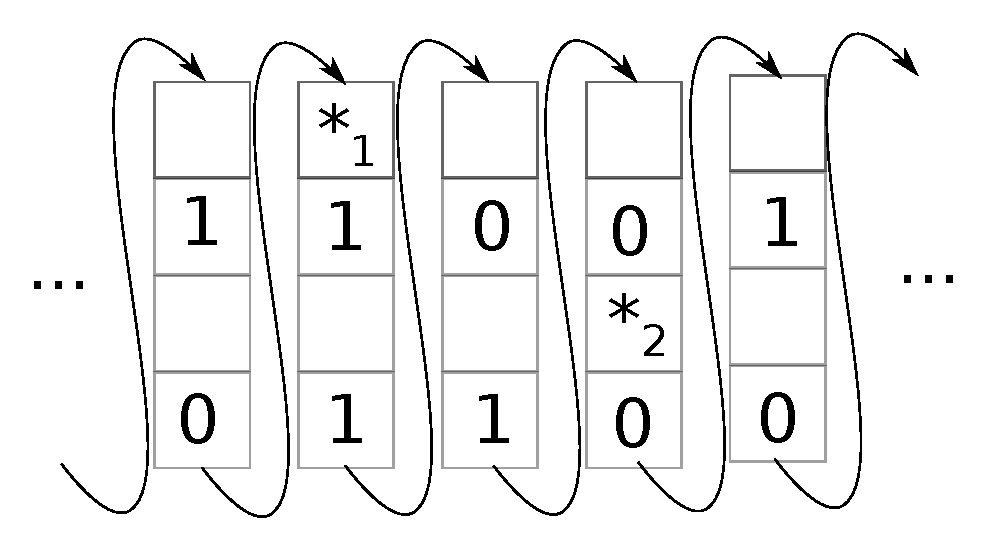
\includegraphics[width=0.49\textwidth]{computability/completeness/pictures/multitape}
		\end{center}
		where the $*_n$ means \emph{tape $n$ is currently at the following value}. 
		
		Now design the states and transitions such that
		\begin{algorithmic}[1]
			\ForAll{tape $t$}
				\State move to the far left.
				\State assume state $(s, t)$, where $s$ is the state of the multi-tape machine.
				\State move right until you find $*_t$.
				\State execute the step, that the multi-tape machine would make.
				\State move $*_t$ left or right, if necessary.
			\EndFor
		\end{algorithmic}
		While this leads to a lot more states, it makes it possible to execute 
		more than one tape simultanously.
	\Question {\tt A;B} inherits the end-states of {\tt B} and the 
		starting-state of {\tt A}. The internal states of {\tt A} and {\tt B} 
		need to be disjunct, otherwise the machine could \emph{jump over} from 
		{\tt A} to {\tt B} or vice versa. To ensure that, we call the states in 
		the new machine $(s, A)$ or $(s, B)$, depending on whether $s$ is from 
		{\tt A} or {\tt B}. Now $\delta((s,A), x) = \delta_A(s,x)$ and
		$\delta((s,B), x) = \delta_B(s,x)$. Finally, we connect the two machines:
		$\forall e\in Endstates_A: \delta((e, A), x) = (start_B, x, N)$
	\Question 
		\subQuestion By the first question, we can assume, that {\tt A}  uses exactly 
			one tape, and also that it is different from the one, that {\tt B} 
			uses. Use a similar construction as with the last question:
			\[\forall e\in Endstates_A: \delta((e,A), (\_, T)) = (start_B, (\_, T), (N, N))\]
			and
			\[\forall e\in Endstates_A: \delta((e,A), (\_, F)) = (end, (\_, F), (N, N))\]

			To round things up, connect the ends of {\tt B} to the $end$ state.
		\subQuestion
			Add the following constraint:
			\[\forall e \in Endstates_B: \delta((e,B), \_)= (start_A, \_, (N, N))\]
	\Question
		\subQuestion We introduce the turingletters $\turingletter{nil}, \turingletter{cons(},
			\turingletter{)}, \turingletter{,}$ to the alphabet. Now given two tapes, we first 
			write our return value on a third (empty) tape: first write
			$\turingletter{cons(}$ moving right, then we copy the first tape and add
			$\turingletter{,}$. Finally we copy the second tape and close with $\turingletter{)}$.
			Note here that {\tt cons} and its friends are part of the \WHILE language,
			and $\turingletter{cons(}$, \dots are letters we can put on a tape of a turing
			machine. 
			\subQuestion Here we get a tape on which 
			$\turingletter{cons(}\dots\turingletter{,}\dots\turingletter{)}$ is stored. The problem here is 
			that we need to consider the nesting of {\tt cons}. For this, we use an 
			auxillary tape $aux$ and write a simple stack. 
		\begin{algorithmic}[1]
			\State write $x$ and move to the right on $aux$ if the current input is $\turingletter{cons(}$.
			\State move left on $aux$ if the current input is $\turingletter{)}$.
			\State start copying input to output after encountering $,$.
			\State halt when the $aux$ tape reaches a blank after moving left.
		\end{algorithmic}
			The machine for {\tt hd} then is analogous.
	\subQuestion 
		\begin{algorithmic}[1]
			\ForAll pairs $p$ on the tape
			\EndFor
		\end{algorithmic}

\end{Answer}

These two exercises show, that $\WHILE\epower\TM$. This is important, since 
when showing something to be \WHILE-complete, we don't need to implement the 
\WHILE, but can use \TM instead, which is much simpler.

\subsection{The Halting Problem} \label{sec:halt}
We saw in the introduction, that there are problems, that can be solved in
\WHILE, that can not be solved in \FOR and also that serveral formalisms are
equally powerful to \WHILE, so that one can wonder, if this literally solves
all problems.

Unfortunately, a simple cardinality argument shows that this is not the case: 
There are only countably infinitely many \WHILE programs, as there are only 
so many finite strings, some of which are also \WHILE programs.

The set of functions $\N \rightarrow \N$ however is bigger, as every freshmen 
course in mathematics will show, therefore, there must be some functions that
can not be computed with \WHILE programs. This proof is unsatisfying, as it
does not give a problem that can't be solved. In fact, we would again describe
problems in a finite way, so the argument is mood.

There are however many problems that can explicitely stated but not solved by 
any algorithm. The perhaps most notoric is the halting problem:

\begin{theorem}[Halting Problem]
	There can be no program $\mathtt{halt?}\in \WHILE$ such that 
	\begin{align*}
		\interpret{\mathtt{halt?}}&:\WHILE\times \Input[\WHILE] \longrightarrow \{True, False\}\\
		\interpret{\mathtt{halt?}}&(p, i) \peq\begin{cases}
			False, &\text{ if }\interpret{p}(i)=\bot\\
			True, &\text{ else}
		\end{cases}
	\end{align*}
	So $\mathtt{halt?}$ answers if a given program with a certain input will halt.
\end{theorem}
\begin{proof}
	The proof is a variation of the quintessential uncomputability proof: We 
	assume that we had $\mathtt{halt?}$ and construct a program, that leads to a
	contradiction. The program is a variation of {\tt inverse}:

	\begin{verbatim}
		loopInverse read P {
		  if [halt?](P.P) {
		    while True { }
		  }
		} write P
	\end{verbatim}

	So we should get
	\begin{equation*}
	 \interpret{loopInverse}(p) = \begin{cases}
			\bot, &\text{ if }\interpret{p}(p) \neq \bot\\
			p,& \text{ else} 
		\end{cases}
	\end{equation*}
	what then is $\interpret{loopInverse}(loopInverse)$? Either it loops or it 
	returns, so lets first assume that it loops:

	\begin{align*}
		\interpret{loopInverse}(loopInverse) &= \bot &\Rightarrow \\ 
		\interpret{halt?}(loopInverse) &= False &\Rightarrow \\ 
		\interpret{loopInverse}(loopInverse) &= loopInverse\neq \bot
	\end{align*}

	So on the other hand, what if it didn't loop?

	\begin{align*}
		\interpret{loopInverse}(loopInverse) &\neq\bot &\Rightarrow \\
		\interpret{halt?} &= True & \Rightarrow \\
		\interpret{loopInverse}(loopInverse) &= \bot
	\end{align*}

	Therefore no such \WHILE program can exist.
\end{proof}

Lets reflect on this proof: While it does use \WHILE, it would be easy to 
translate {\tt loopInverse} into other languages and give a halting 
problem for those. In fact, if we can compile {\tt loopInverse} into a 
language, then the new language can not solve its own halting problem, even 
if it was more powerful than \WHILE.

\begin{corrolary}
	No language at least as powerful than \WHILE can solve its own halting problem.
\end{corrolary}

\subsection{Rice's Theorem}
\label{Rice}
Now maybe the Halting Problem is very special and maybe we're not even that 
interested in the halting of the machine. Maybe we're interested in another 
property $P$, for example ``if the machine halts, its result is the fibonacci 
frequence" or ``the machine leaves this part of the memory untouched".

Such procedures would certainly be useful for specification, security, etc.\ but
Rice proved in 1953 that these procedures cannot exist either.

\begin{theorem}[Rice]
	If there is a property 
	\[ P: (\Input[\WHILE]\rightarrow \Output[\WHILE])\rightarrow \{True, False\}\] 
		such that there are procedures $x$ and $y\in \WHILE$ such that 
		$P(\interpret{x})=True$ and $P(\interpret{y}) = False$ then there can be 
		no procedure $\interpret{p}: \WHILE \rightarrow \{True, False\}$ that corresponds to $P$.

		So if we have a non-trivial property of functions, we cannot write a
		program, that can deduce if the property holds based on the source of a
		procedure alone.
\end{theorem}
\begin{proof}\TODO\lineofthought{What do the sub-programs do exactly}
	We can easily see that the halting problem is a special case of this, but 
	in fact, with a simple construction, all cases come down to it.

	First we note that a procedure $\interpret{z}(x)\peq \bot \forall x$ must 
	either have the property $P$ or not. Since $p$ halts, we can check that in 
	advance. Assume that $\interpret{p}(z)=False$, then we can build a program 
	that can solve the halting problem:

	\begin{verbatim}
maybe-p: read (Q.I.X) {
  [interpreter](Q,I)
  Y := [known-p](X)
} write Y

halt: read (Q,I) {
  known-p-or-z := [spec](maybe-p.Q.I)
  Y := [p](known-p-or-z)
} write Y
\end{verbatim}
	The trick here is that 
	\[
		\interpret{\interpret{spec}(\mathtt{maybe-p}, \mathtt{Q}, \mathtt{I})}(x)\peq \begin{cases}
			\interpret{z}, &\text{ if } \interpret{Q}(I) \peq \bot\\
			\interpret{known-p}, &\text{ else }			
		\end{cases}
	\]
	
	and therefore 
	$\interpret{\mathtt{halt}}(q,i)\peq True\Leftrightarrow \interpret{\interpret{spec}(\mathtt{maybe-p}, \mathtt{q}, \mathtt{i})} \peq \interpret{\mathtt{known-p}}\Leftrightarrow$
	$\interpret{q}(i)$ halts and vice versa for the contrary case.
\end{proof}

\subsubsection{So how do we deduce properties about programs then?}
Rice tells us, that it is not possible to deduce for example, 
that the result of a computation is a {\tt String}. Yet the Java compiler 
does it all the time. How is this possible?

The trick is that Rice tells us that the problem can't be solved \emph{in full
generality}. So instead of accepting all programs, we accept only the ones for
which we \emph{can} prove the property. This throws away an infinitude of
perfectly reasonable programs, which would keep the property, only because we
can't prove it, but this way, we can be sure that for any program we accept,
the property \emph{does} hold.

\subsection{The Normal Form Theorem}
\begin{theorem}[Normal Form Theorem]
	Every \WHILE program can be transformed into a \WHILE program with exactly 
	one {\tt while} loop. That is, all the inner constructs are taken from \FOR.
\end{theorem}
\begin{proof}
	Lets call the language of \WHILE programs, that are in the normal form $\WHILE_1$.
	We have seen that we can transform $\WHILE \rightarrow \TM$ and 
	$\TM \rightarrow \WHILE_1$. If we chain these (informal) compilation processes to 
	get a compiler $\WHILE \rightarrow \WHILE_1$.
\end{proof}

\subsection{Church's Thesis}
As mentioned, when the notion of computability was first developed, there 
were competing formalisms, but as it turned out, they were all equally 
powerful. This lead Alonzo Church to conjegure, that what the human sees 
as intuitively computable, is adequately formalized by any of these 
competitors. This is known as Church's Thesis (or Church-Turing Thesis).

\begin{thesis}[Church's Thesis]
	The Turing Machine adequately models what we hold for intuitively computable.
\end{thesis}

We saw that \WHILE too is a competitor, since it is equally powerful to any 
of the other formalisms. We could then formulate it as follows:

\begin{thesis}
	There is no intuitive extension of \WHILE that is more powerful than \WHILE.
\end{thesis}

For example, we could add procedure calls, but that would not make any 
functions computable that were not computable before.

The thesis can not be formally proven, since it connects the informal concept 
of ``intuitively computable" with the formal Turing Machines, however the 
evidence that no-one has since build a computer, that could be exploited to
calculate more than a \TM gives a strong indication, that the Church-Turing
Thesis is true.

\subsubsection{\dots or is it?}
There has been some work, what would happen, if you added certain 
functionalities to Turing Machines (and by extension to \WHILE). 

Turing himself analysed so-called oracle machines, which are basically Turing 
Machines, but can answer specific questions to an oracle on a different tape, 
that would answer if a specific predicate is true for the value of the tape.
The halting problem for Turing Machines is not solvable on a normal \TM, but 
we could add an oracle for it. This would be more powerful than \TM, but it 
is not intuitively clear how one could build such an oracle. Also, we would 
find, that the oracle machine could not solve its own halting problem -- for 
very much the same reason that the original \TM can't solve its own.

Another line of thought is that, when we talk about these formalisms, we 
don't really care if humans find it intuitively computable, but rather that 
we could actually build a machine that computes it. This gives us the 
physical Church-Turing thesis: It is not possible to build a computer that 
can not be simulated on a \TM.

This is a thesis, that \emph{can} be put to the test. While \TM rely on 
classical mechanics, some thought has been put into quantum computing. The 
model that is currently used to build quantum computers (qubits) are however
not stronger than \TM. Faster yes, but not really stronger.

On a larger scale, it is possible to construct a computing device that orbits 
around a rotating black hole. An observer falling into the black hole could 
then observe the infinite computation time of the orbiting machine in
subjectively finite time\footnote{See \cite{etesi2002blackhole} for the whole
discussion on the feasability and the mathematical proof}. It has however been
noted, that falling into a black hole might not be a good idea\citationneeded.

Finally, the notion of a computer running and halting after some time might 
be flawed. There is no procedure, that can compute $\pi$ to its full extend, 
but many approximation procedures, which can give a arbitrarily precise 
result. Is $\pi$ then intuitively computable?

\subsection{Properties of Turing complete languages}
There are some common elements in the languages that are Turing complete. As we
have seen, any Turing complete language is unable to solve it's own halting
problem -- and by extension any halting problem of a Turing complete language.

Often, it is not obvious, that a certain formalism is Turing complete.

\subsubsection{Conway's Game of Life}
In 1970, the British mathematician John H. Conway devised a ``game" on an 
infinite squared paper: we start with some squares marked as ``alive" and 
then we update the paper in the following way\footnote{The general machine 
	that updates cells only taking the cells neighbors into account is called a 
cellular automata}:

\begin{itemize}
	\item A dead square becomes alive, if it has exactly three 
		neighbors\footnote{diagonal cells are neighbors too},that 
		are alive. Imagine that the cells around it would reproduce and the 
		offspring move into this square.
	\item If the cell is alive, it stays alive if only if it has two or three 
		living neighbors.
\end{itemize}

These extremely simple rules still make up a turing complete language. How 
could one guess that it was?

The first hint is the discrete infinite data structure. We have an unlimited (but 
never infinite) number of squares that are alive. 

This is a necessary condition to be Turing complete. Imagine, that we only
allow a limited data structure, for example a Turing tape that has $n$ cells
and an alphabet of $k$ letters. Each cell has therefore only $k$ possible
configurations, and all the cells combined have only $k^n$ possible states.
Since our machine only has a limited number of states, it can be in, say $m$,
and the head has only $n$ posible positions to be in, after at most 
$n\, m\, k^n$ steps of the machine we must have reached a state that we have
seen before.  The transition function does only depend on these factors,
therefore the loop will start again and nothing new will come of it.

Another hint is that there is no obvious way to deduce certain properties 
without running the whole machine -- ``Is this cell alive after $n$ turns" 
can only be anwered after running $n$ turns.

The real test is of course to implement a turing machine in the game of life, 
but this is beyond the scope of this 
text\footnote{\url{http://rendell-attic.org/gol/tm.htm} has an 
implementation of a turing machine in the Game of Life}.

\paragraph{Why are most programming languages Turing Complete?} % (fold)
\label{sub:Why are most programming languages Turing Complete?}
Not being able to tell if a program will stop nor any other interesting 
properties seems like a bad start. Further, we use mostly algorithms that are
guaranteed to hold in finite time. In short, we seldom truly need a Turing 
complete language, but still every major programming language is Turing 
complete. 

The reason for this is that programmers don't want to think about the halting 
of their programs, because normally they obviously do. Proving that might not 
be trivial and might require the programmer to rewrite the program in such a 
way, that a computer can prove it. So while it would be possible to to 
implement most algorithms in a weaker language, it would be impractical. We
couldn't use any unboundedd loop constructs or true recursion.

In some areas, this is acceptable: In formal logic and interactive 
proof-finding, Coq\footnote{\url{http://coq.inria.fr/}} is used, eventhough it has 
no unbounded recursion and every piece of code terminates.
% subsection Why are most programming languages Turing Complete? (end)
